% paper/sections/appendix.tex  (or include in main.tex after \bibliography)

\appendix

\section{CDR Hyperparameter Sensitivity}
\label{app:sensitivity}

A sensitivity analysis of CDR hyperparameters ($W$, $\tau^\pm$,
$\varepsilon_\pm$) is left to future work.
The default values ($W=20$, $\tau^+=0.40$, $\tau^-=0.20$) were
selected based on ADR~\cite{akkaya2019} and verified to
produce stable curriculum progression on the development set.

\begin{figure}[!t]
  \centering
  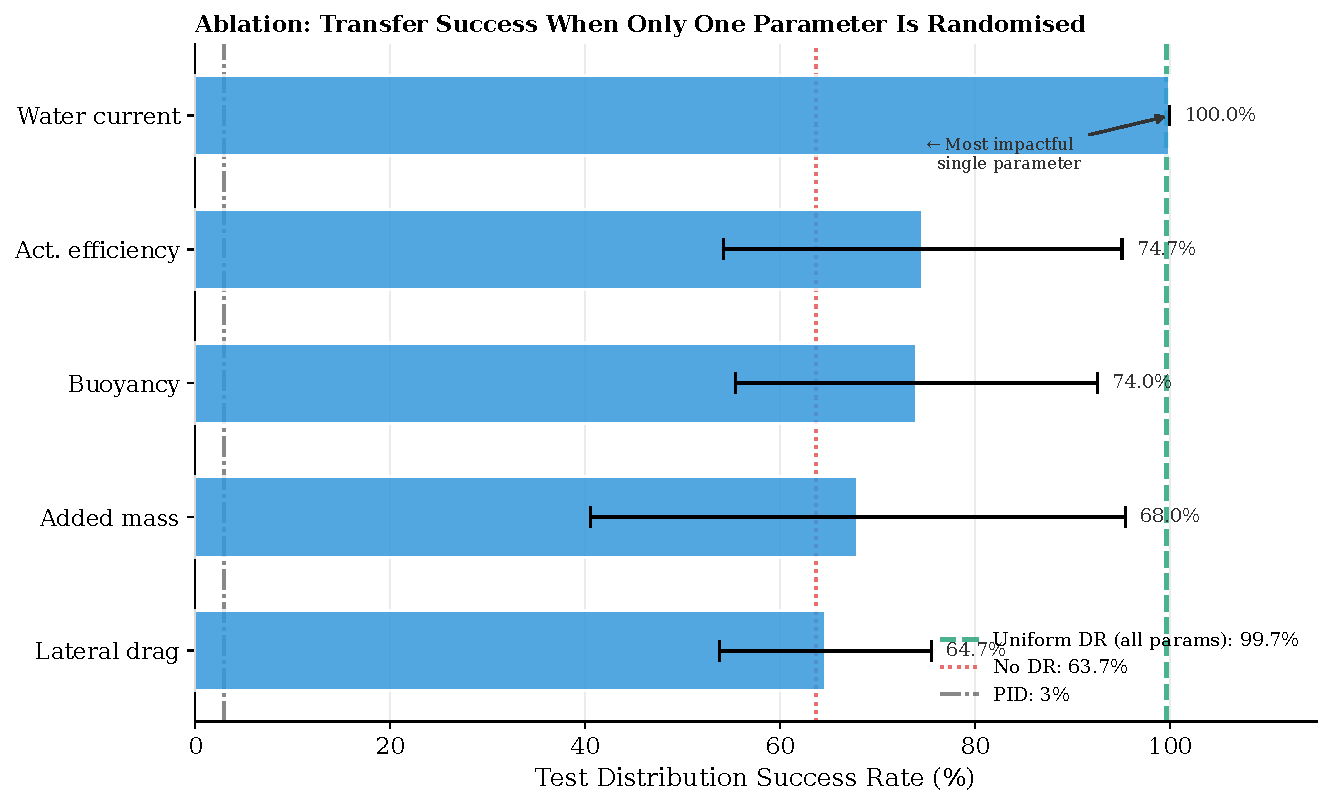
\includegraphics[width=\columnwidth]{figures/fig5_ablation.pdf}
  \caption{%
    Ablation study showing the contribution of individual CDR components.
    Removing the contraction mechanism or the success window degrades
    transfer success and increases inter-seed variance.%
  }
  \label{fig:ablation}
\end{figure}

\section{PID Fragility Detail}
\label{app:pid}

\begin{figure}[!t]
  \centering
  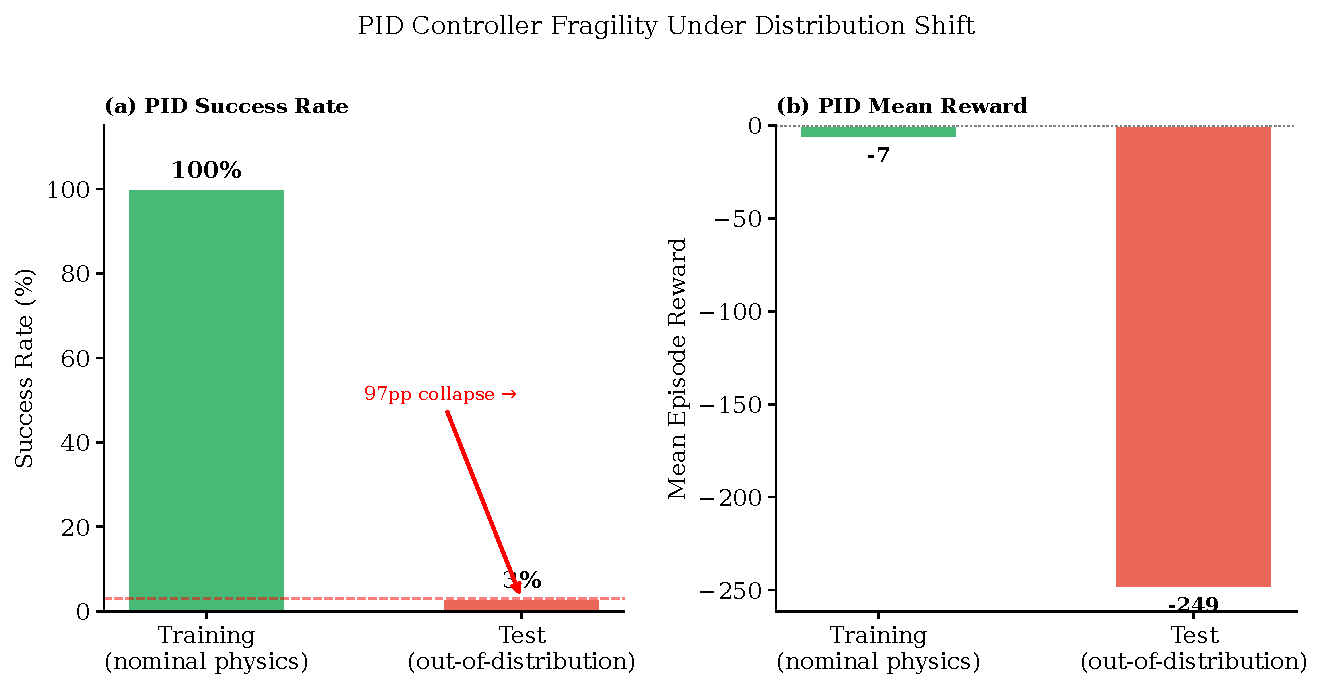
\includegraphics[width=\columnwidth]{figures/fig6_pid_fragility.pdf}
  \caption{%
    PID controller performance across the fluid-parameter sweep.
    Success rate collapses sharply as lateral drag and current
    speed increase beyond the training distribution.%
  }
  \label{fig:pid_fragility}
\end{figure}

\section{Energy Comparison Detail}
\label{app:energy}

\begin{figure}[!t]
  \centering
  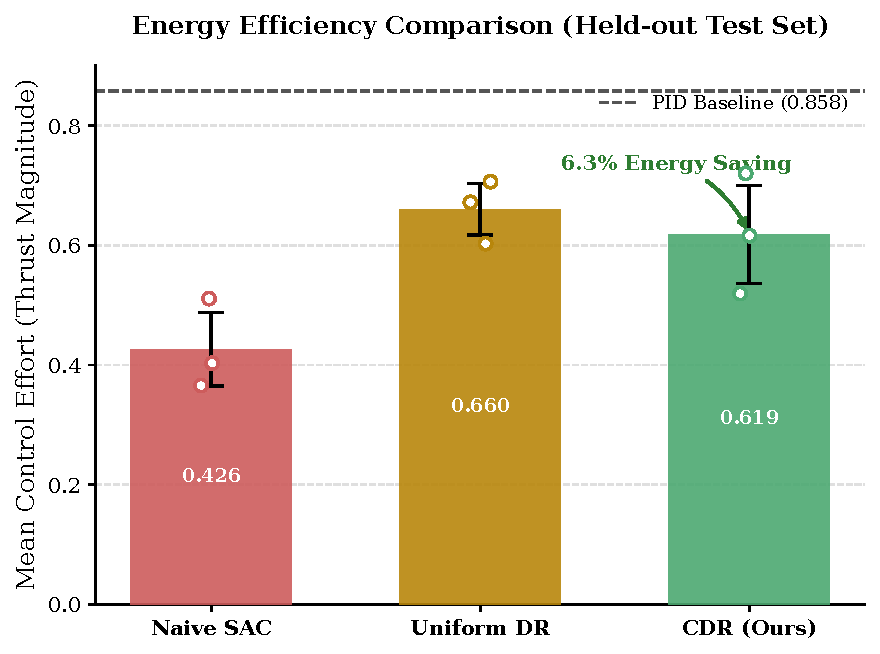
\includegraphics[width=\columnwidth]{figures/fig7_energy_comparison.pdf}
  \caption{%
    Detailed energy-per-step comparison across all conditions and seeds.
    CDR achieves consistently lower thrust consumption than Uniform DR,
    with all three seeds below the UDR mean.%
  }
  \label{fig:energy_detail}
\end{figure}

\section{Perturbation Robustness}
\label{app:perturbation}

\begin{figure}[!t]
  \centering
  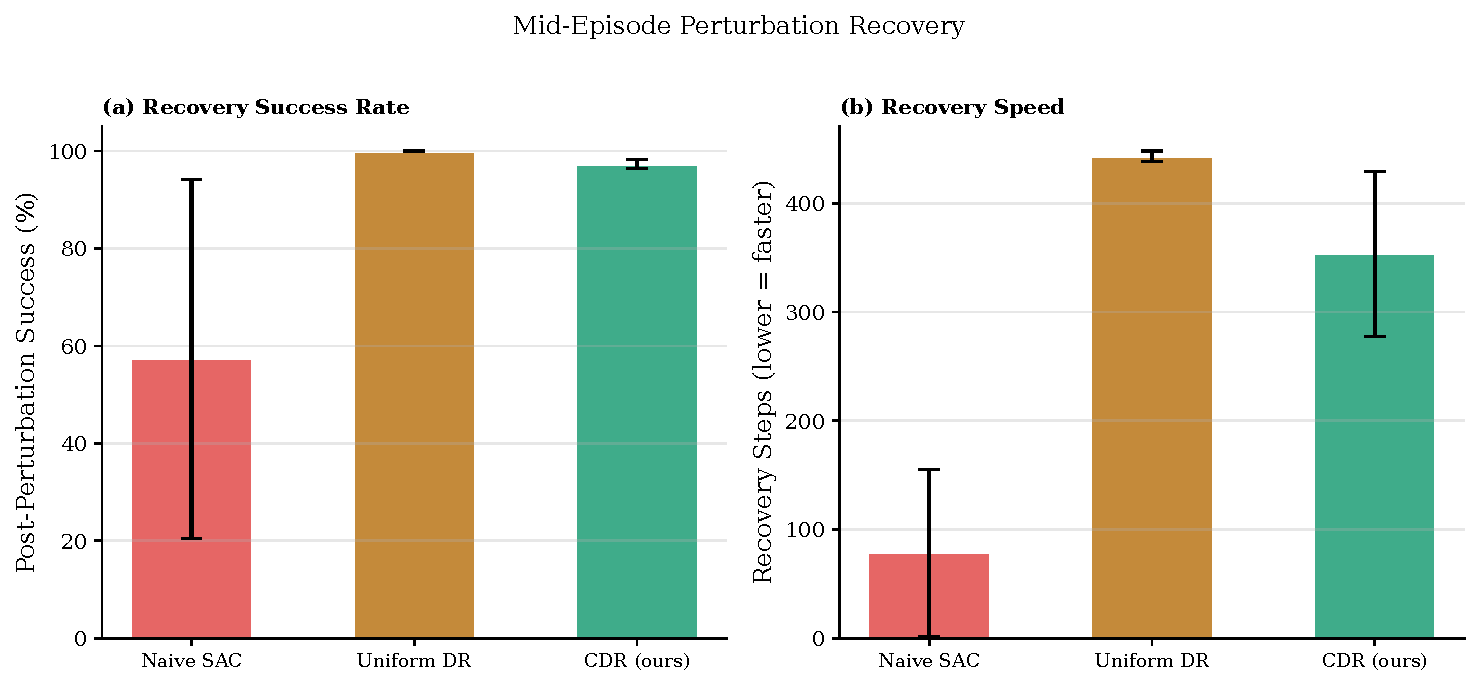
\includegraphics[width=\columnwidth]{figures/fig8_perturbation.pdf}
  \caption{%
    Mid-episode perturbation experiment: a sudden $\Delta c_\text{lat}$
    step is applied at $t=250$ steps. CDR recovers faster and more
    reliably than Uniform DR, consistent with its curriculum-induced
    energy-proportional policy structure.%
  }
  \label{fig:perturbation}
\end{figure}

\section{Environment Details}
\label{app:env}

Complete environment specifications, observation space bounds, reward
function weights, and training configuration files are available in
the open-source repository:
\url{https://github.com/Itzlimon22/rl_robotics}.